

\chapter{Casi d'uso}                %crea il capitolo
%%%%%%%%%%%%%%%%%%%%%%%%%%%%%%%%%%%%%%%%%imposta l'intestazione di pagina
\lhead[\fancyplain{}{\bfseries\thepage}]{\fancyplain{}{\bfseries\rightmark}}
Di seguito alcuni esempi di utilizzo della libreria.
Le dimostrazioni seguenti sono state effettuate su una macchina con architettura amd64 e con installato il sistema operativo debian in versione sid (quindi unstable) ma sono state testate e riprodotte anche su altre configurazioni e distribuzioni GNU/Linux.
\section{Environment}
Come precedentemente accennato possiamo integrare la nostra libreria in vuos attraverso il modulo unrealvsnlib o creandone uno alternativo che dipenda da VsnLib.\\
\begin{description}
\item[Creazione moduli:] La creazione di un modulo \`e molto semplice e basta serguire le linee guida di quelli preesisteni, inoltre grazie ad una routine in cmake non \`e necessario aggiungere alcuna riga manualmente al makefile e sar\`a, appunto, cmake ad occuparsi della compilazione.
\item[Start Vuos:] Vuos si avvia attaverso il comando umvu ed \`e in grado di interpretare comandi successivi come argomenti, come mostrato nell'esempio infatti umvu \`e affiancato dal comando xterm e pertanto verr\`a lanciata una nuova istanza di terminale con ambiente vuos. Nel caso specifico \`e stato utilizzato il programma konsole, Il risultato non cambia; in alternativa anche bash o zsh andrebbero bene ma si perderebbero le informazioni mostrate da vuos nel primo terminale.
\item[Include dei Moduli vuos] I moduli in vuos vengono inclusi attraverso la direttiva
\begin{verbatim}
vu_insmode <nome_modulo>
\end{verbatim}
Un esempio di avvio e inclusione del modulo \`e quello della figura seguente.
\begin{figure}[h]                       %crea l'ambiente figura; [h] sta
                                        %   per here, cio� la figura va qui
\begin{center}                          %centra nel mezzo della pagina
                                        %   la figura
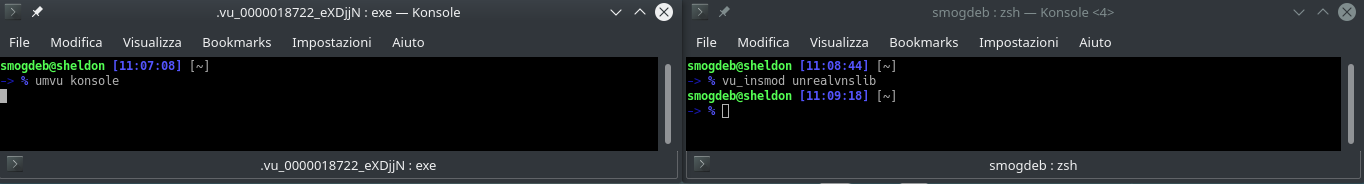
\includegraphics[width=16cm]{start_vuos}%inserisce una figura larga 5cm
                                        %se si vuole usare va scommentata
%
%%%%%%%%%%%%%%%%%%%%%%%%%%%%%%%%%%%%%%%%%inserisce la legenda ed etichetta
                                        %   la figura con \label{fig:prima}
\caption[start/include\_mod vuos]{start and include vuos}\label{fig:map}
\end{center}
\end{figure}
\end{description}
\section{Esempi}                 %crea la sezione
Nella parte successiva verr\`a mostrato un esempio di configurazione per LWIPv6 attraverso VsnLib.\\
Per motivi di chiarezza e completezza si \`e deciso di non utilizzare l'ambiente sopra descritto o altre tecniche di cattura delle system call ma i pacchetti netlink sono stati costruiti all'interno del codice di test. Sono esempi statici di come li creerebbe il programma ip ma utili a mostrare sia come \`e formato un pacchetto di questa tipologia sia per tracciare i passi compiti per il parsing e la configurazione.
\begin{description}
\item[Init VsnLib: ]L'unico header di riferimento della libreria necessario \`e vsnshared.h, all'interno troviamo dichiarate le funzioni necessarie all'utilizzo della libreria.
\begin{lstlisting}[style=CStyle]
extern int init_vsnlib(char* stack);
extern void handle_vsnlib(void* buf, size_t len, void* nif, void* stack);
\end{lstlisting}
La prima funzione serve per indicare alla libreria di quale modulo fare il load pertanto richiede come input il path del file da caricare.
La seconda \`e l'unico ``handle'' per passare il pacchetto netlink che dovr\`a essere poi interpretato, inoltre prende come argomeni anche un puntatore allo stack e all'interfaccia oggetto della modifica.
\item[Strutture: ]I pacchetti netlink sono accomunati dallo stesso header, come mostrato in precedenza, ma presentano strutture diverse per il resto. In questo esempio sono stati creati i pacchetti per l'aggiunta e la rimozione di un indirizzo da un'interfaccia, l'aggiunta e la rimozione di una rotta e l'accensione/spegnimento di un'interfaccia.
\begin{lstlisting}[style=CStyle]
struct info{
  struct rtattr attr;
  unsigned char ip6_address[sizeof(struct in6_addr)];
};

  struct addr_payload{
  struct nlmsghdr header;
  struct ifaddrmsg ifa;
  struct info attribute[2];
};

struct route_payload{
  struct nlmsghdr header;
  struct rtmsg rtm;
  struct info attribute;
};

struct link_payload{
  struct nlmsghdr header;
  struct ifinfomsg ifi;
};

\end{lstlisting}
rispettivamente:
\begin{itemize}
  \item info contiene il payload con gli indirizzi.
  \item addr\_payload viene usato per aggiungere/rimuovere un indirizzo da un interfaccia.
  \item route\_payload usato per aggiungere/rimuovere rotte.
  \item link\_payload per attivare/disattivare l'interfaccia.
\end{itemize}
La descrizione \`e ristretta a questo esempio, ma queste strutture vengono impeigare per compiere pi\`u azioni di quelle presentate.
\item[Creazione pacchetti: ]\`E eseguita dalle funzioni nel test.
\begin{lstlisting}[style=CStyle]
void fill_buf_addr(struct link_payload* buffer, int mode);
void fill_buf_route(struct link_payload* buffer, int mode);
void fill_buf_link(struct link_payload* buffer, int mode);
\end{lstlisting}
Il compito di queste funzioni \`e riempire i campi delle strutture sopra elencate in base all'operazione richiesta, \`e possibile modificarle per ottenere comportamenti diversi e compiere altri test.\\
In pratica si occupano di fare quello che farebbe un programma come ip in maniera semplificata, questo rende pi\`u semplice al lettore la comprensione, la modifica e l'utilizzo degli strumenti proposti.
\item[VsnLib: ]Per tutte le operazioni viene chiamata sempre la stessa funzione ``handle'' di VsnLib cambiando solo il paccehtto inviato di fatto. Questo dimostra come la libreria sia in grado di interpretare in maniera autonoma i pacchetti netlink ed utilizzarne le informazioni per completare con successo (o con fallimento in caso le informazioni non siano coerenti) le operazioni richieste.
\item[Test: ]Ispirato da un programma esplicativo per LWIPv6 questo test dovrebbe avere lo stesso comportamento di netcat ma la configurazione dello stack avviene attraverso VsnLib e i pacchetti netlink, come mostrato nell'Appendice \ref{code:AppB}.
Andiamo in sequenza:\\
Come prima operzione viene inizializzata VsnLib, successivamente controlla che non sia necessario caricare LWIPv6 dinamicamente ed una volta superato questo step vengono creati stack e interfaccia di rete (nel caso specifico viene collegata ad uno switch vde). In ultima analisi vengono eseguite le configurazioni necessarie a rendere l'interfaccia attiva.
\item[Replica dell'esperimento: ]
\end{description}
%%%%%%%%%%%%%%%%%%%%%%%%%%%%%%%%%%%%%%%%%non numera l'ultima pagina sinistra
\clearpage{\pagestyle{empty}\cleardoublepage}
